This chapter provides a theory which stands behind Apache Flink and Kafka Stream,
key concepts and illustrative examples, and main challenges.
A reader should be able to understand a context and why such frameworks needed.
Both frameworks are based on principles of distributed systems design, which
all be covered in context of a given problem.

\section{Why framework is needed}\label{subsec:why-framework-is-needed}
During the research, I've figured out is that lots of engineers or developers who
have never worked on data engineering problems have a narrow overview about
what actually data frameworks are needed for.

Let's define a simple task which is given by a business, for example business wants to know
what songs get more streams in different countries.
A very simple solution would look like the code below.

\subsection{Simple pipeline example}\label{subsec:simple-pip}
\begin{lstlisting}[label={lst:chart_list}]
    top_charts = db.select("top_charts")
    ordered_bands = top_charts
        .groupBy(chart -> chart.country)
        .agreggate_by(chart -> chart.streams)
        .order_by(chart -> chart.streams)
        .map(chart -> {chart.streams, chart.song, chart.country})

    dashboard.show(ordered_bands)
\end{lstlisting}

At first look, it works as business wants and the question of why framework is needed for,
is still not clear, because a simple script would do this job well enough.
But here is coming a tricky part, what if data volume has become extremely large
which leads a slow execution time, and for some reason application start getting OutOfMemory exception.
It this case, the pipeline gets down and business goal is now achieved.

A first solution which comes to mind, is just to run separate jobs for different country ranges and
then combine results.
To run it such way that each script would become as independent deployable application
which contains almost the same code, or can be the same if country ranges are specified as
input parameters.

\begin{lstlisting}[label={lst:chart_list_2}]
    top_charts = db.select("top_charts").where(europe)
    ordered_europe_bands = top_charts
        .groupBy(chart -> chart.country)
        .agreggate_by(chart -> chart.streams)
        .order_by(chart -> chart.streams)
        .map(chart -> {chart.streams, chart.song, chart.country})

    dashboard.show(ordered_europe_bands)
\end{lstlisting}

This solution might help for some time, if data is still growing then
it would become a nightmare supporting many similar jobs and
then implementation additional jobs which combines results from all jobs
and sends it to centric dashboard.
Many jobs also would require additional devops setup and time.
Also, it's not that ease to implement parallelize a job, if to run a job in parallel
then they would produce the same result, just independently.
Moreover, problems with processing speed and memory exertion can come back.

\begin{description}
    \item[Scalablity] it's quite clear that a solution with a simple script is not scalable
    for huge datasets.
    \item[Devops] requires additional work for development team, if case of trying to run
    the same job but for different country ranges.
\end{description}

There's a solution for such cases, frameworks which are designed for such cases.
Moreover, they provide an api which
look almost the same as map, filter, reduce functions.

Here are key points about frameworks for data pipeline, which do much more under
the hood comparing to a simple script.

\begin{description}
    \item[Scalablity] It's scalable by default, just by specifying config.
    The main different in scalability is that frameworks use models such as
    MapReduce, DAG.
    It means that frameworks knows itself how be scalable itself, under the hood,
    using multiple nodes.
    More details about MapReduce and DAG in the next chapter.
    Framework knows how spread sub problems across multiple parallels executors,
    and then combines many results to a one single output.
    \item[Performance] Execution performance is achieved by having multiple
    parallel workers which communicate to each other.
    \item[Fault Tolerance] Frameworks cares about fault tolerance, having a built-in replica
    functionality, where replication is self organized by a framework.
    \item[Kubernets operator] Modern frameworks provide Kubernetes operators to
    manage deployment which significantly simplify developments.
    \item[Cumminty Support] All modern frameworks provide a great support which
    \item [Built-in integrations] For example it can be machine learning, external data sources,
    graph processing algorithms.
    dramatically helps in setting up a cluster or a code implementation.
\end{description}

\subsection{Simple pipeline example with Apache Spark}\label{subsec:simple-spark}

With a framework the pipeline looks the same, but with having all these features
provided in the list above.

\begin{lstlisting}[label={lst:spark}]
spark = SparkSession.builder
    .appName("Country Musical Streams")
    .getOrCreate()

df = spark.read.csv(data_path)
result = df.groupBy("country")
    .agg(sum("streams").alias("total_streams"))
    .order_by(chart -> chart.streams)
    .map(chart -> {chart.total_streams, chart.song, chart.country})

\end{lstlisting}

Obviously, frameworks have some disadvantageous, in case a big data
it's the only way to go.
Some of disadvantageous are:

\begin{description}
    \item[A need in learning new technology] A developer who's has to develop a data pipeline
    has to understand what he's doing, how it works, and how to properly use an api.
    \item[Deployment Setup] It's different comparing to a simple application.
\end{description}

Frameworks allow to reuse already existing pipelines and make relly reliable
and scalable solution.
This is just a small example to imagine how it's used and why.
The next chapter goes to a technical details more deeply.


\section{Stream processing: concepts}\label{sec:-concepts}
%First at all, I'm providing a key difference between a batch processing and a stream processing.
%
%In a batch processing mode, a job works with a data which has a defined size, for example,
%database records, csv file.
%It reads a date, process it and provides a result.
%
%Batch processing jobs usually get executed periodically with 3 main states,
%which are, startup,

A stream has a very broad mining, for some people it refers to
C++ standard input/output library, for some file stream and
for an average person it would mean video content stream, for example
on YouTube or on Twitch.
An actual meaning of a stream for a context of data processing
is subsequent flow of an immutable data records or messages.
A record or a message are interchangeable in this context.

A typical stream processing is an implementation of a generic producer/consumer pattern.
Producer/consumer pattern is quite similar to publisher/subscriber pattern but there's
a difference between these two patterns.

\textbf{Publisher/Subscriber} is mostly used for a one-to-many communication,
such as notifications or push messages.

\textbf{Producer/Consumer} is used for a one-to-many, one-to-one and many-to-many,
many-to-one communication.
Is used with messages queues.

It is important to know that a difference between these patterns might be tricky,
lots of details depend on a certain pattern implementation.
For example, Apache Kafka uses producer/consumer, but Apache Pulsar uses published/subscriber.
Both can be used for a data streaming, it is important to figure out what does a business
actually want, before developing a solution.

\subsection{Dataflow graph}\label{subsec:dataflow-graph}
This is the core part which confuses lots of developers who are not familiar
with data processing frameworks.
In the previous chapter, two scripts with a data pipeline were provided, where
one uses a standard language api and another is written with Apache Spark.
Such frameworks like Apache Spark, Apache Flink and Kafka Streams actually
use dataflow graph model under the hood, to achieve a high performance and parallelism.
Just implementations might be slightly different.

Since some developer wind parallelism quite challenging to
understand, not just a parallelism itself by rather a model
its evolution, how did the data systems get to this moment.
It's actually an evolution log research which has taken decades and
it's quite complicated to imagine what's going to be next evolution
in data streaming systems.

\begin{description}
    \item[Dataflow Architectures] In 70s, researchers were looking for new approach in
    designing parallel computing systems.
    These prototypes represented computations in directed graphs,
    where nodes were operations and edges indicated data dependencies.
    These prototypes allowed to achieve an asynchronous and fine-grained parallelism,
    which was a departure from the conventional von Neumann architecture.
    Some notable dataflow machines from this era include the Manchester Dataflow Machine,
    MIT's VAL, and the Japanese ETL-Mark-III.
    \item[Dataflow Programming Languages] Next step was between 70-80s.
    First dataflow programming languages were developed to handle parallel programming challenges.
    These languages, such as Id, SISAL, and Lucid, used dataflow principles
    to express parallelism explicitly and manage dependencies between operations.
    This allowed developers to focus on application business logic rather on parallelism
    while the runtime system took care of scheduling and synchronization.
    Obviously there were that advanced as modern programming languages as java or C++, but it
    was a significant progress.
    \item[Dataflow Models for Parallel Processing] Further research on dataflow models moved
    focus from hardware architectures to software-based dataflow models,
    which enabled a higher level of abstraction and portability.
    Some of these models, like the Bulk Synchronous Parallel (BSP) and LogP,
    influenced the design of parallel programming libraries and frameworks, such as MPI and PVM.
    Progress in new languages programming languages such C/C++ a more advanced hardware did
    a big step to focus more on software models.
    \item[Dataflow Models for Data Processing] This is a modern era of dataflow models in distributed computing.
    Dataflow models gained renewed interest as a way to represent and reason about data processing pipelines.
    Systems like Google's MapReduce, Apache Hadoop, and Apache Spark adopted dataflow
    concepts to enable large-scale data processing in distributed environments.
    MapReduce gave a huge step forward for modern data processing frameworks, however,
    MapReduce is getting less popular due popularity of Apache Flink and Kafka Steams which
    adopted MapReduce and dataflow model for a real time stream processing.
    At the moment dataflow graphs as a core component for modeling real-time data processing pipelines,
    which provides a great performance in an ease in use by provide a high-level api.
\end{description}

This brief history gives a high-level overview about moder data processing system to
understand a main difference between running a simple script or running on top of
data processing framework.

Figure \ref{fig:dataflow-graph} shows how a data frameworks uses graphs
to process a stream in parallel.
Each parallel process gets executed in its own graph which allows to achieve high
parallelism level.

\begin{figure}[H]
    \centering
    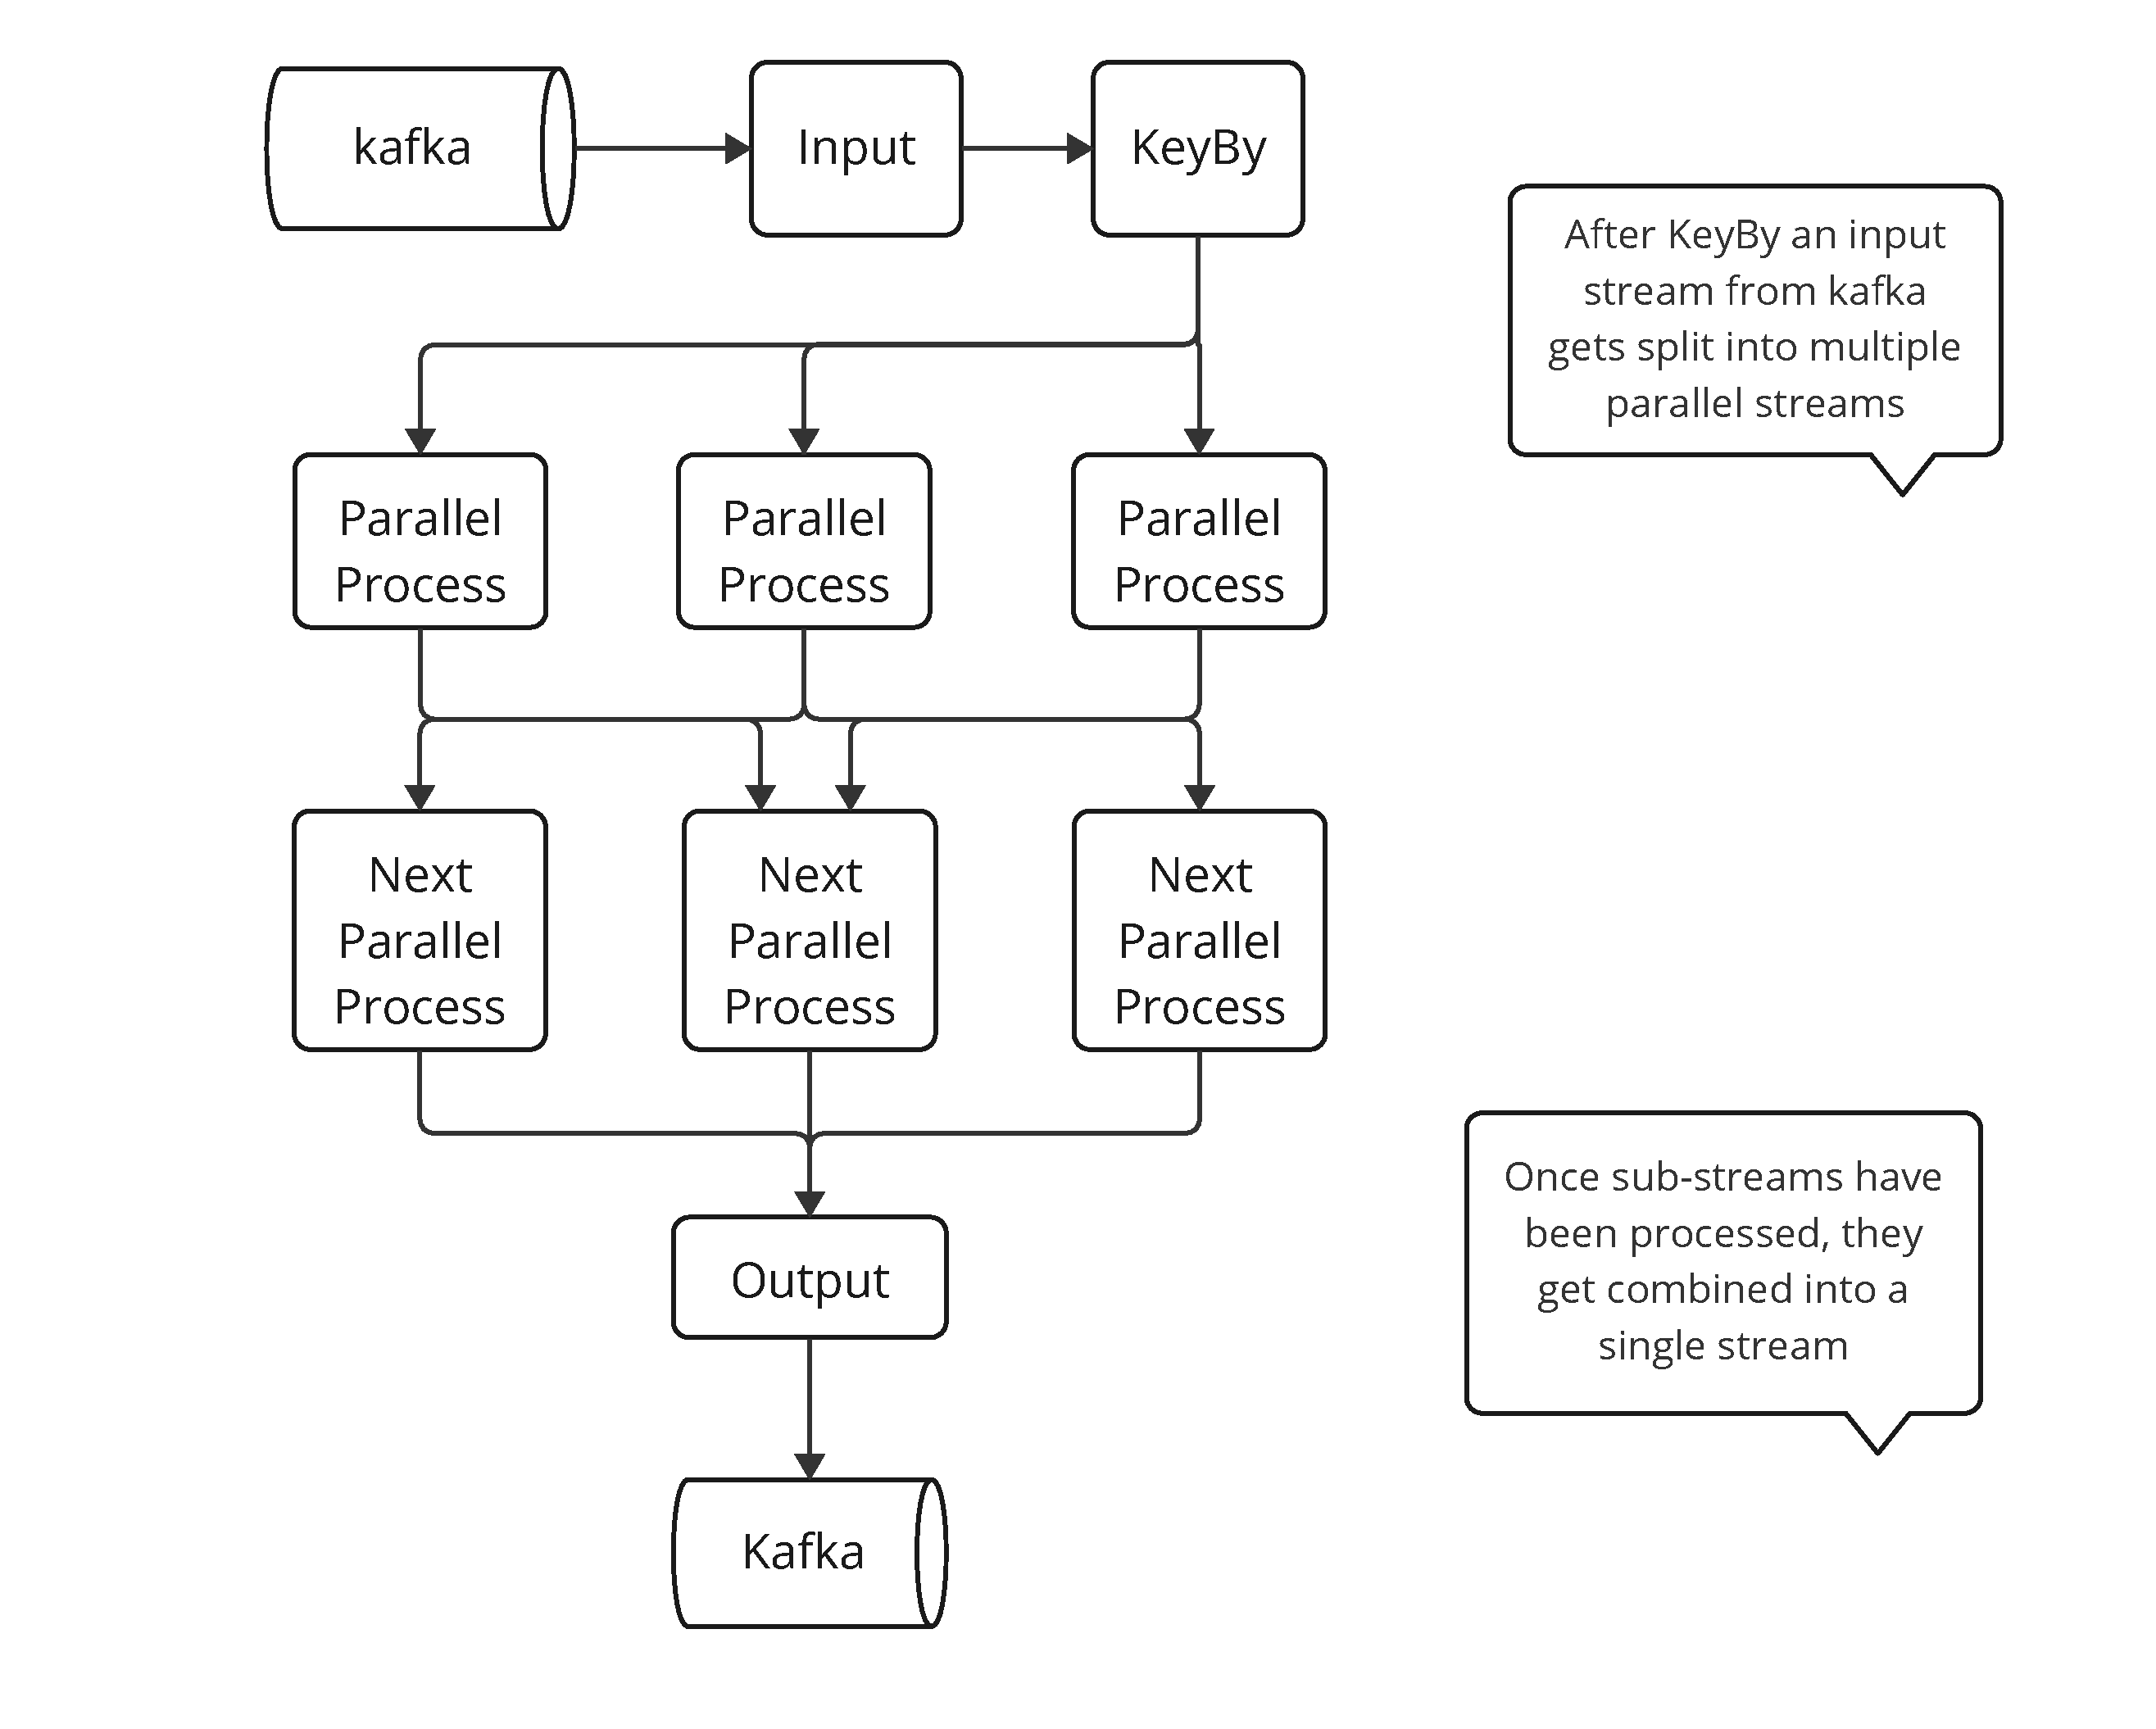
\includegraphics[width=1\textwidth]{figures/dataflow-graph}
    \caption{\textit{An example of data stream execution with dataflow graphs.}}
    \label{fig:dataflow-graph}
\end{figure}

\newpage

\subsection{Data Parallelism and Task Parallelism}\label{subsec:data-parallelism-and-task-parallelism}
Data parallelism and task parallelism might sound confusing even for experienced developers.
In dataflow graphs, parallelism can be achieved in two ways.
Data parallelism with partitioning input data and executing tasks of
the same operation on data subsets in parallel, allowing for efficient processing
of large data volumes and spreading the computation load across multiple computing nodes.
Task parallelism, on the other hand, refers to tasks from different operators
performing computations on the same or different data in parallel,
which enables better utilization of the computing resources in a cluster.

\begin{figure}[H]
    \centering
    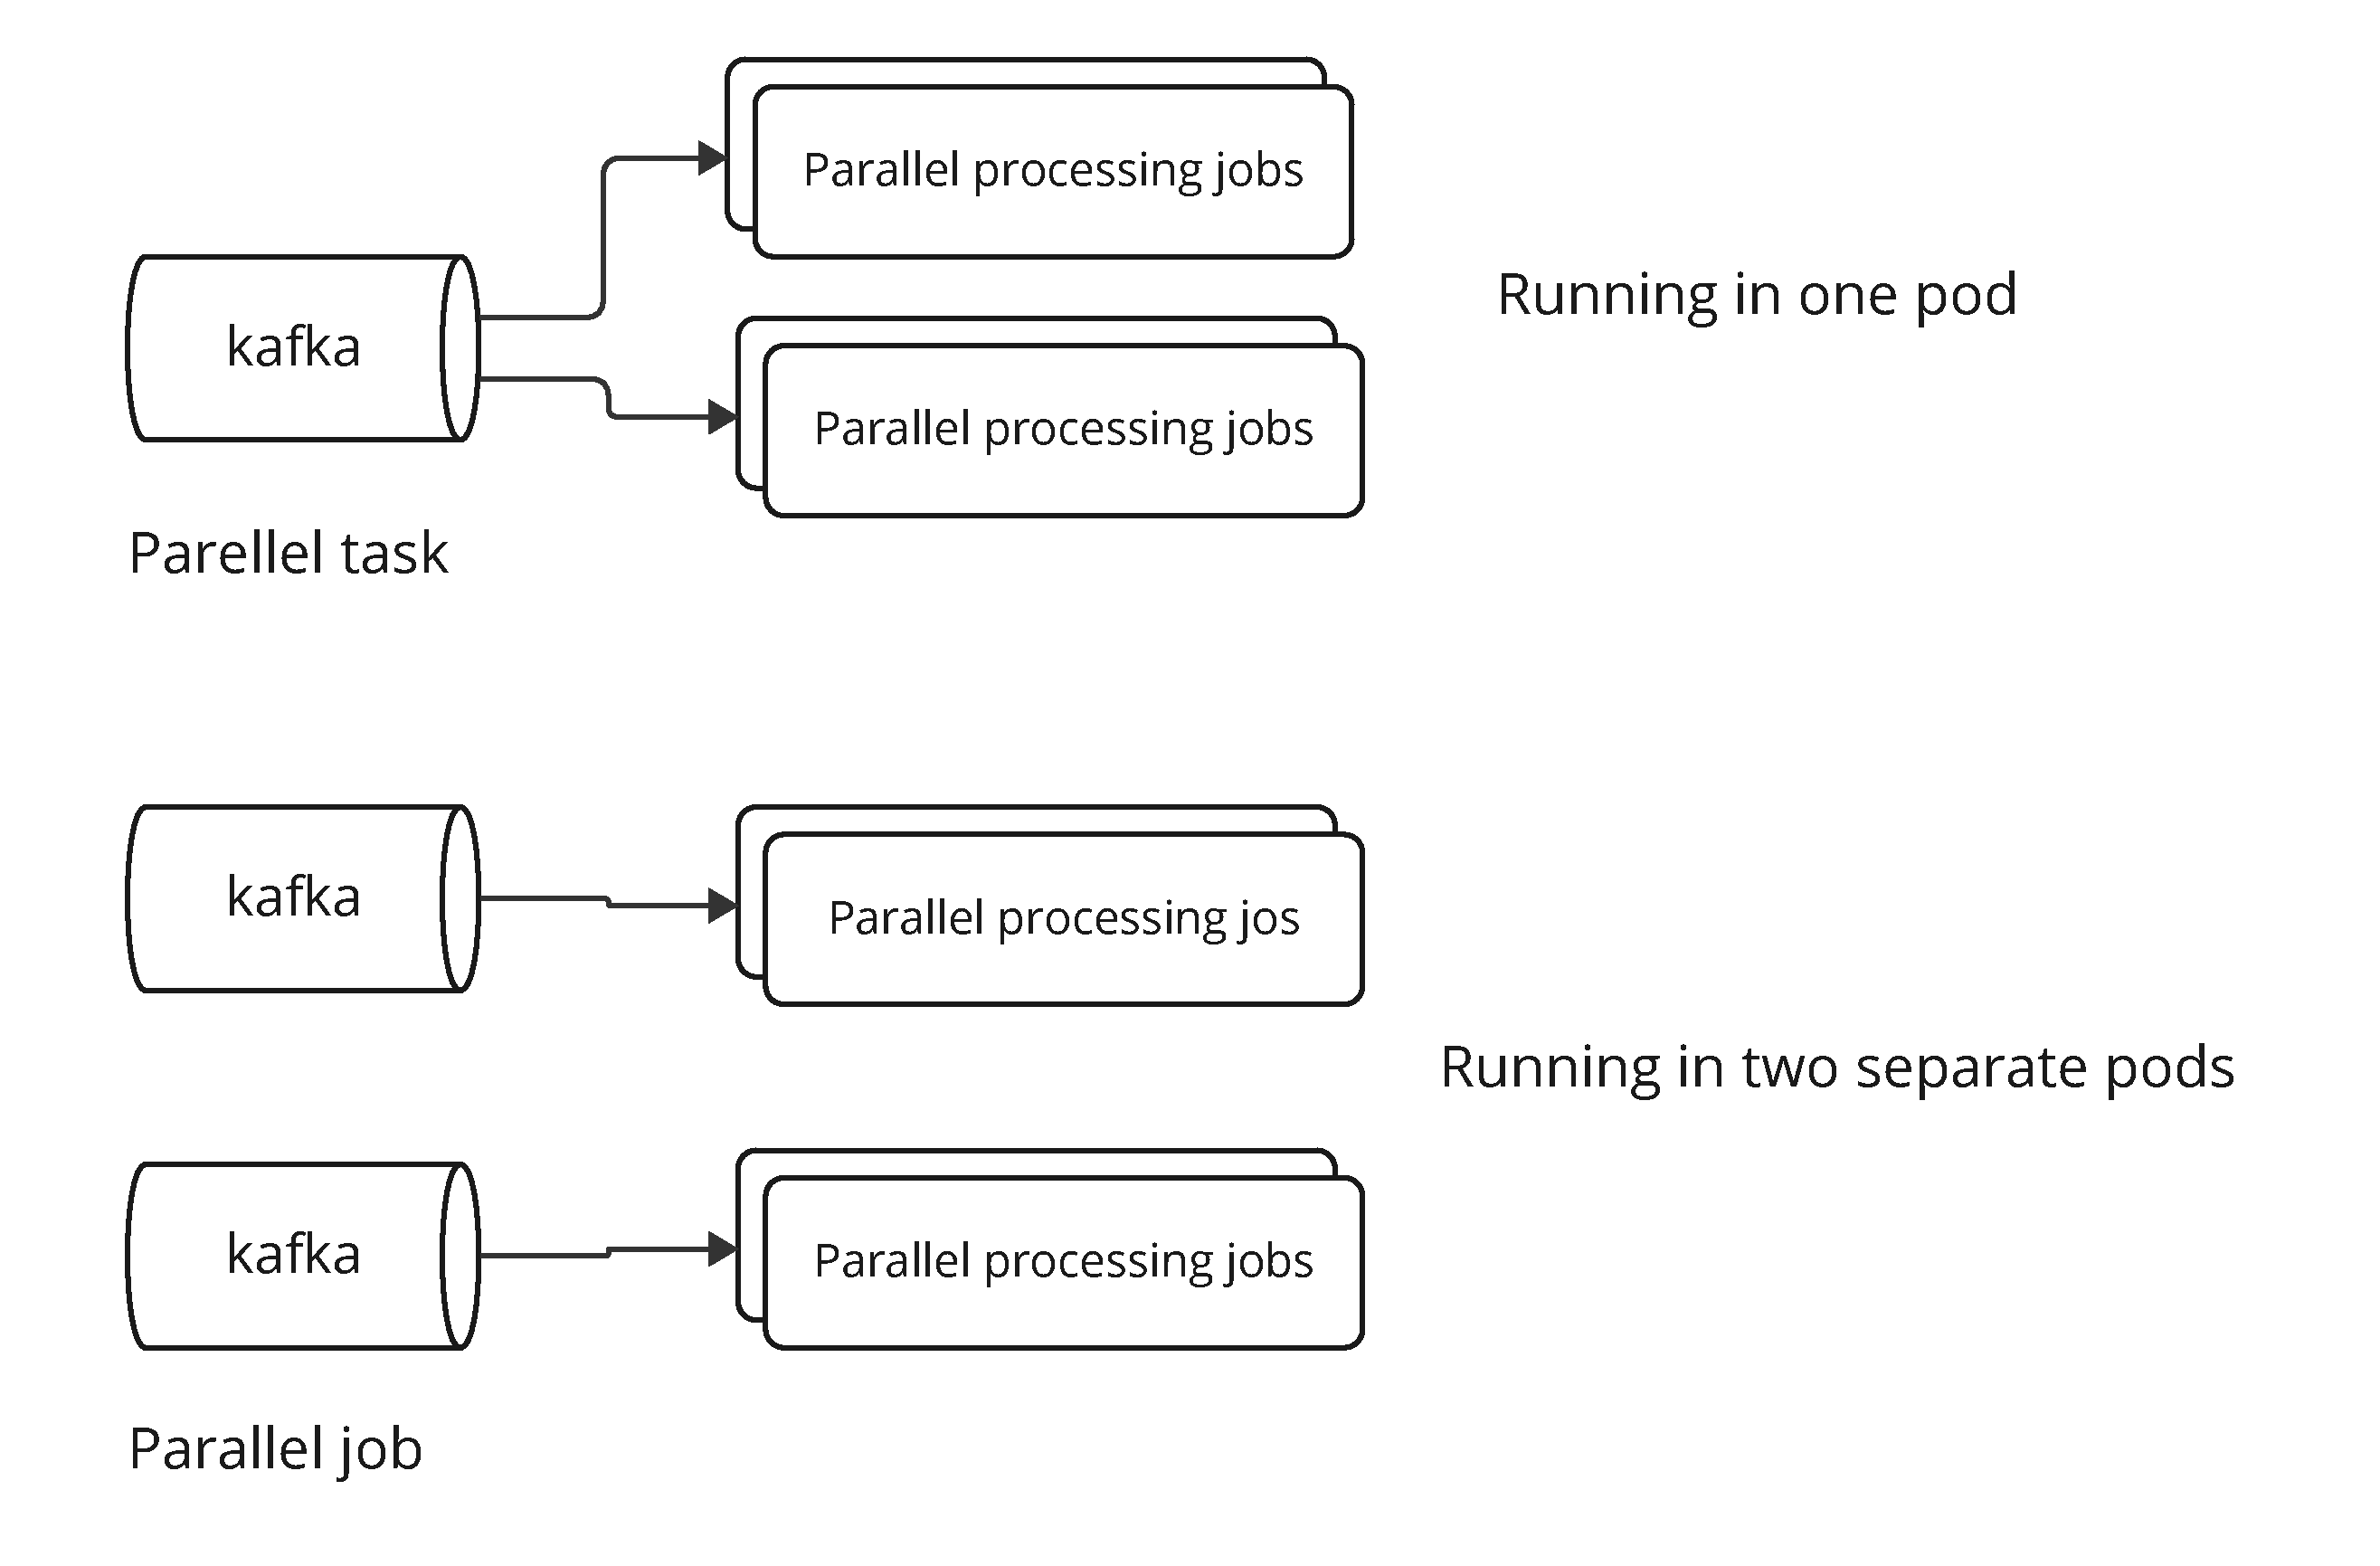
\includegraphics[width=1\textwidth]{figures/parallel-jobs}
    \caption{\textit{An example of data stream execution with dataflow graphs.}}
    \label{fig:parallel-job}
\end{figure}

In order to get better understanding, Figure \ref{fig:parallel-job} depicts a visual difference.
Job parallelism defined how many parallel task are running in separate execution node,
but performing as one single app.
In case of Kafka, each job's task processes a subset of kafka partitions, such
that all tasks process all partitions.
Kafka knows how to spread partitions among all tasks, a developer
don't need to worry about it, only if there's a very specific case for that.
In general partitioning should work automatically, the only a number of partitions
is under developer's responsibility.
There's a formula which defined a number of partition for a project which is getting started,
but as a data volumes grow it's good practice to add more partitions manually.
Moder monitoring tools help to identify such moment, when a number of partitions
should increase to handle new data volumes.

\subsection{Data Exchange Strategies}\label{subsec:data-exchange-strategies}

\begin{description}
    \item[Forwarding] The forwarding approach passes data straight from one task
    to the downstream task without reshuffling or rearrangement.
    The downstream operator processes data in the same sequence and partitioning
    as the upstream operator.
    Forwarding is the most efficient strategy, due to less overhead and network communication.
    \item[Partitioning] Data is redistributed among parallel jobs depending on a key or function.
    Key-based partitioning, which shuffles and groups data by key values, is the most frequent.
    Keyed aggregations, joins, and groupBy use this method.
    Partitioning processes all records with the same key.
    \item[Broadcast] Data from upstream jobs is replicated and delivered to downstream activities.
    In a broadcast join or when a small dataset needs to be available to all downstream
    for processing, then broadcast strategy is used.
    \item[All-to-All] The all-to-all technique sends all upstream records to all downstream jobs.
    This method is utilized when data order or partitioning doesn't matter
    or when every task must process the complete dataset.
    For large datasets, this method has a substantial transmission overhead.
    \item[Rebalancing] Rebalancing redistributes data evenly across downstream processes.
    It prevents data skew and load imbalance from uneven data distribution.
    Rebalancing guarantees that downstream tasks receive roughly the same quantity of records,
    improving performance and resource use.
    \item[Random] Random uniform distribution across downstream tasks.
\end{description}


\begin{figure}[H]
    \centering
    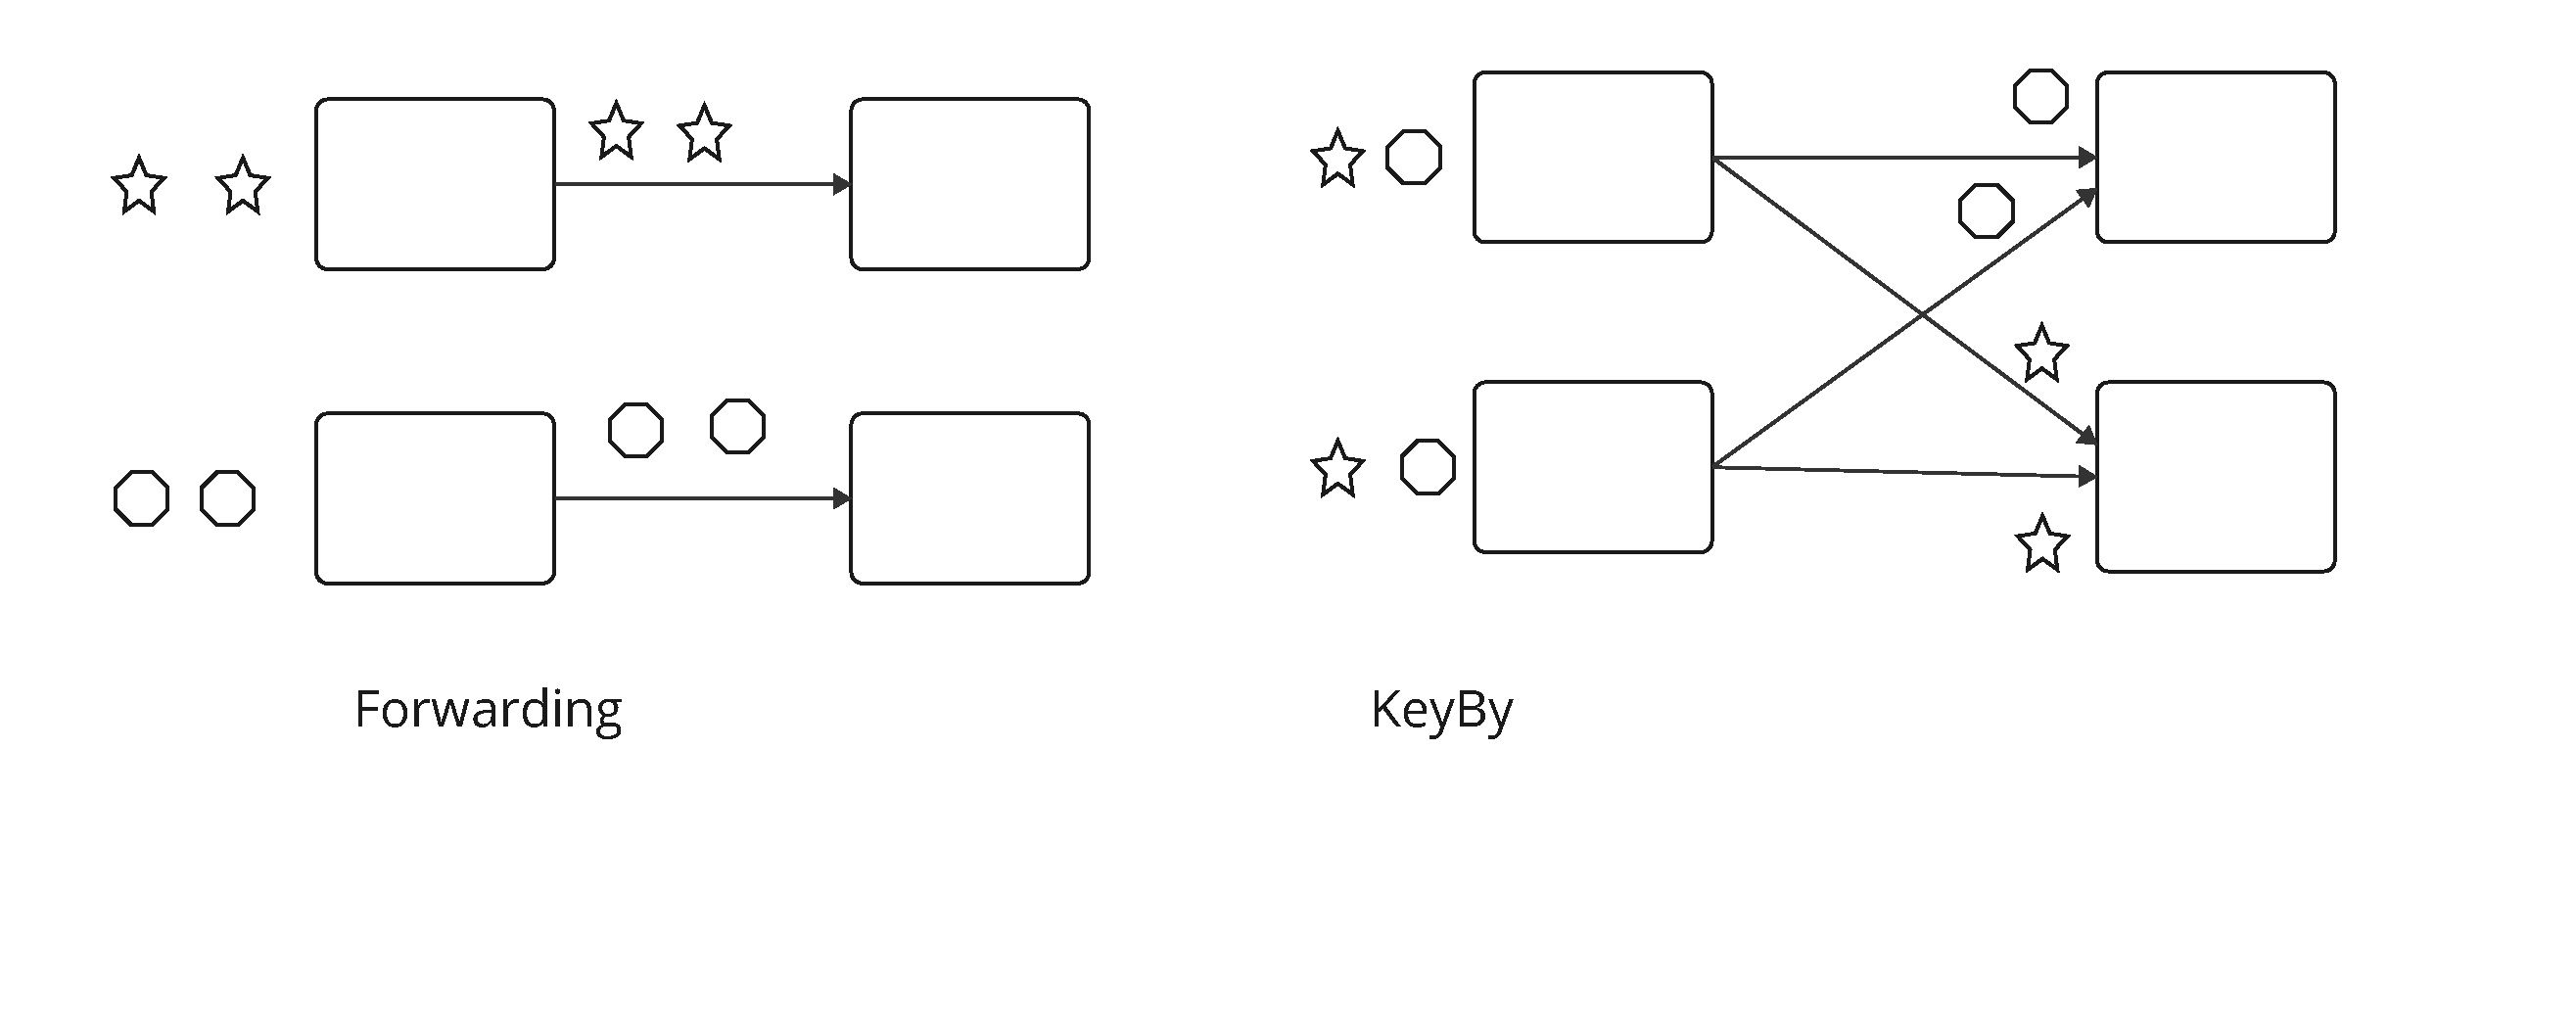
\includegraphics[width=1\textwidth]{figures/forward}
    \caption{\textit{An example of forwarding and partitioning by key.}}
    \label{fig:forward}
\end{figure}

\newpage
\section{Stream processing: challenges}\label{sec:-challanges}
Since this research is focusing on stateful streaming,
a variety of challenges must be handled by a new solution.

\begin{description}
    \item[State Management] In the following context, a state represents a unit of information
    which can saved, accessed and updated by a key.
    For example a key based counter.
    In a distributed streams,
    updating and accessing state might be difficult.
    Operators must ensure consistency and minimal latency while managing
    state across multiple jobs and nodes.
    In order to handle state efficiently, sharding, partitioning,
    and replication must be used.
    \item[Fault tolerance] fault tolerance was already covered earlier as a requirement.
    It's also quite challenging since different frameworks have different strategies for 
    recovery.
    \item[Scalability] Scalability also was covered earlier as a requirement, scalability
    as a fault tolerance are done differently for streaming frameworks.
    \item[Rebalancing] Balancing is a core feature which deals with fault tolerance
    and scalability the same time.
    There are difference options, which are configurable.
    Kafka provides a great api for a flexible setup.
    In this case it's important to sync with business requirements.
    Balancing will be covered in details in the next chapter.
    \item [Processing latency] It is challenging, both Apache Flink and Kafka Stream are able
    to handle a load in a reasonable time range.
    \item[Exactly-once semantics] This challenge depends on a use case.
    Since exactly-once semantics is solvable with some tradeoffs  with a kafka, it
    will be covered in details in next chapters.
    \item[Deployment] At this time, streaming frameworks have already Kubernetes
    integration which allows to manage deployment and resources.
    Still some details might be challenging, like auto-scaling.
    At the beginning data processing frameworks were designed for deployment
    on YARN cluster.
    Step by step data frameworks have migrated to Kubernetes.
\end{description}

These challenges are most the important in this research, and in order to
understand how they can be solved I'll provide more details in the next sections.
Details for these challenges will be explained on top of the use case.

\newpage
\section{Kafka as a stream data provider}\label{sec:kafka-as-a-data-provider:-challenges}
The use case which will be evaluated in this research is supposed to work with kafka which
provides a source of unbounded data stream.
Some developers might be confused about terminology and a difference
between kafka and kafka streams.
This section is trying to describe Kafka components and describe what is important
for the thesis research.

\begin{description}
    \item[Kafka] is a distributed messaging system.
    \item[Kafka Streams] is a streaming library which is built on top of Kafka.
\end{description}

From a very generic view Kafka represents a message queue and consists
of 3 core high level components which are Consumer, Producer and Broker.

\subsection{Producer}\label{subsec:producer}
Producer is an application that sends data
records to Kafka topic.
Kafka records can obtain any form of data, including log files, user activity, and sensor readings.
Producers must decide which partition within a topic to send messages to,
either through a round-robin approach or by establishing a partitioning strategy
depending on the message content, for example by record key or by custom balancing strategy.
Kafka provides producer api client which is used withing an application.

\begin{figure}[H]
    \centering
    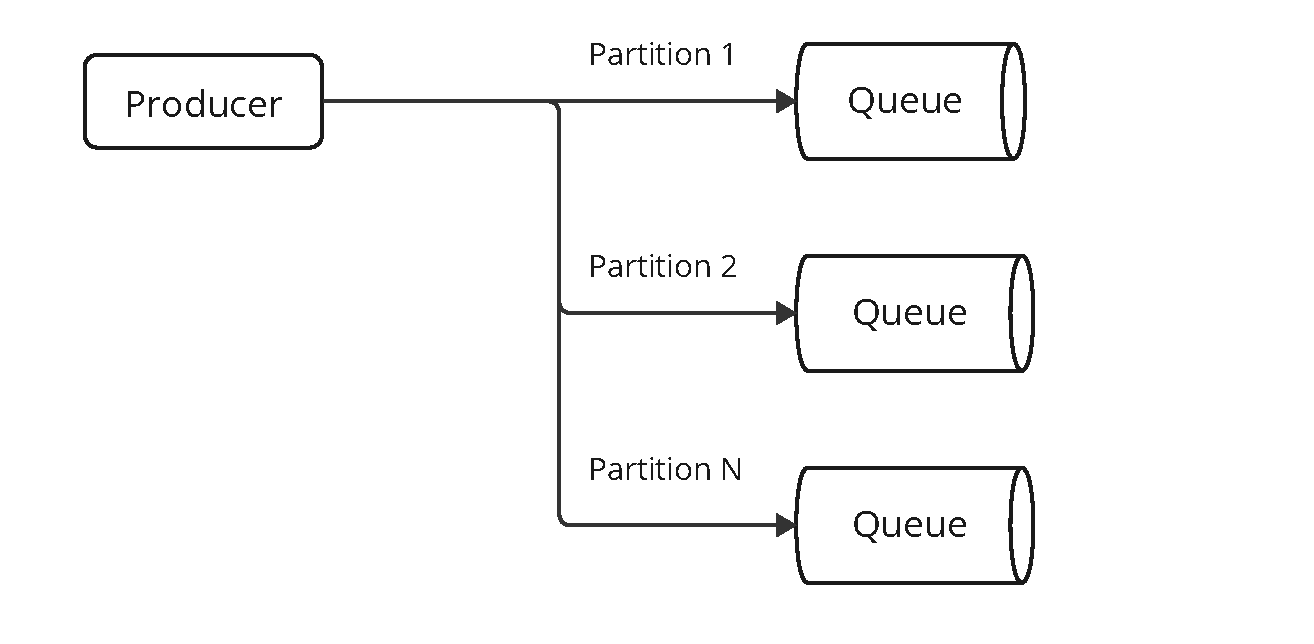
\includegraphics[width=1\textwidth]{figures/producer}
    \caption{\textit{An example of forwarding and partitioning by key.}}
    \label{fig:producer}
\end{figure}

Figure \ref{fig:producer} shows a common producer model which sends
records to Kafka topic which has two partitions.
In case of multiple partitions, Kafka provides multiple
balancing strategist.
A strategy selection depends on a business requirements and a use case.
Down below are described three possible scenarios for balancing.

\begin{description}
    \item[Record key is not specified] In this case producer use Round robin strategy
    and sends records for using each partition subsequently,
    For example, is there are two partitions, first message goes to partition 1,
    seconds to partition 2, third goes to partition 1 and etc.
    \item[Specified partition] A developer explicitly defines a partition to send.
    \item[Partitioning with hash function] Hash function uses a record key as
    an in input parameter hash output specifies a partition.
    Hash function must deterministic, it means that one key has always the same partition.
\end{description}

For the research use case it was decided to go with the Round robin balancing
since a record is supposed to be 1Kb byre array which has no key.
This allows kafka producer to balance records quite efficiently.

\newpage
\subsection{Consumer}\label{subsec:consumer}
[Consumer] is application that consumes messages from Kafka topic.
As with producer, kafka api also provides consumer api client.
Consumers are members of consumer groups, which enable them to share
the processing load and read messages concurrently.
keep track of their progress by saving the offset of the most recent
message they have consumed.
Each message in a partition is given a distinct offset.
In case of balancing, offset has a pointer which indicates which latest record was consumed by
a consumer.
If several consumers consume the same topic then kafka broker creates two offsets for
each consumer


\begin{figure}[H]
    \centering
    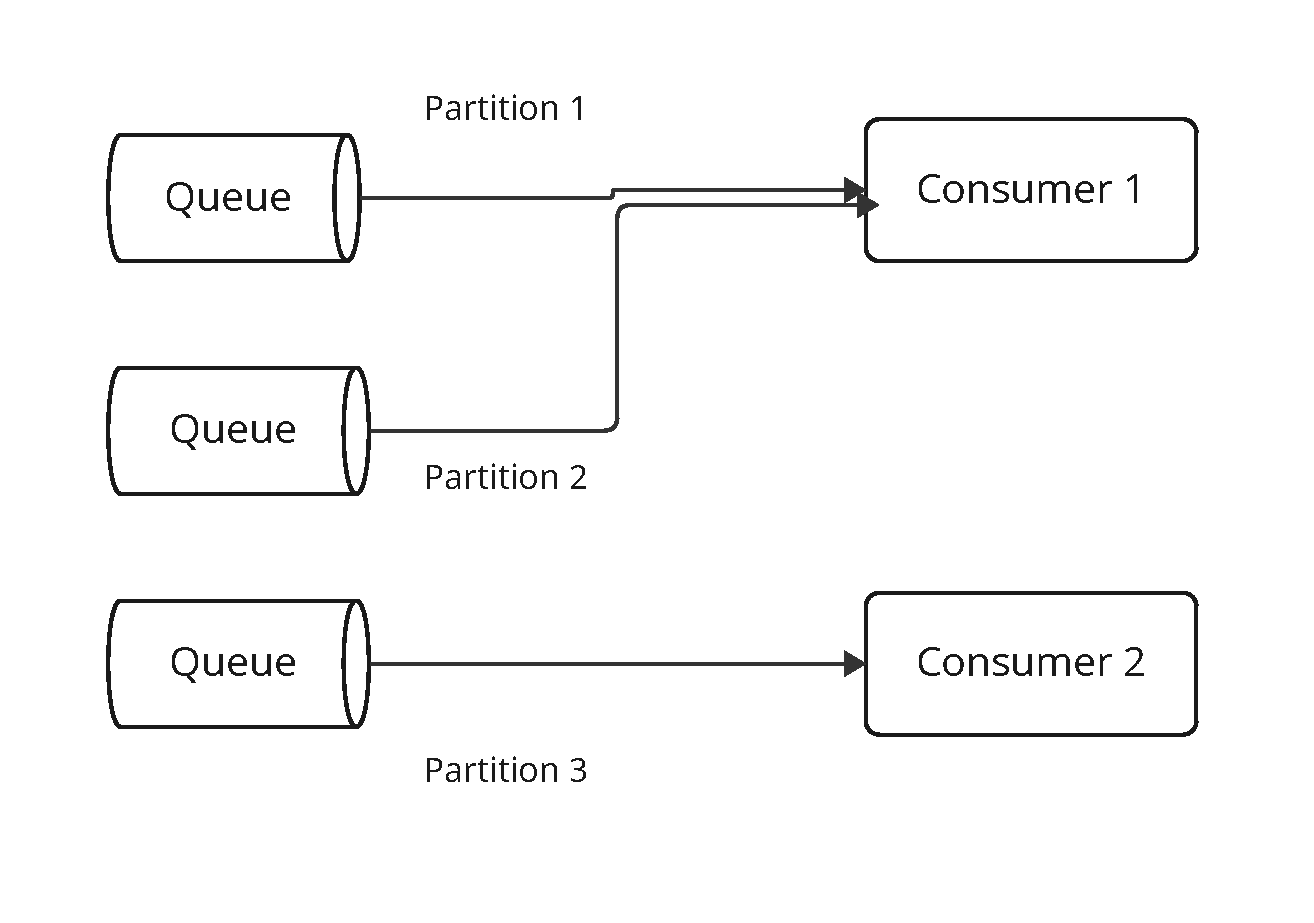
\includegraphics[width=1\textwidth]{figures/consumer-kf}
    \caption{\textit{An example of forwarding and partitioning by key.}}
    \label{fig:consumer-kf}
\end{figure}

Figure \ref{fig:consumer-kf} show a case for three topic partitions and two consumers.
It can be seen that in this case the first consumer consumes two partitions.
In case of one partition, the only one consumer would receive a data stream,
the second would work in idle mode awaiting new available partitions.
Partition assignment is fully managed by the Kafka broker which is described
in the next section.

\newpage
\subsection{Kafka Broker}\label{subsec:kafka-broker}
Kafka broker is a central component of Kafka ecosystem.

Its main responsibilities are:

\begin{description}
    \item[Processing record queus] Each broker manages one or more partitions for each topic.
    When producer sends a record to Kafka topic, the broker stores records
    in the corresponding partitions, which represents multiple queues.
    Each record is assigned to incremental offset within its partition,
    which helps in maintaining the order in which record were written.
    Kafka broker keeps record in a binary format which requires developers
    to implement a corresponding serializer for producer and deserializer for consumer
    if a standard set of serializers and deserializers do not work.
    \item[Replication] To ensure fault tolerance and high availability,
    brokers replicate the data across multiple replicas.
    These replicas are distributed across different brokers in the cluster.
    In case a broker goes down, another broker with a replica of the same data can take over,
    ensuring that no data is lost.
    Replication factor is set by a Kafka cluster administrator.
    \item[Consumer managetment] Broker enable consumers to read records from the Kafka topics.
    The broker makes sure that
    consumers can subscribe to one or more topics and read records
    in parallel by being part of a consumer group, it
    helps consumers track their progress by maintaining
    the offset of the last consumed record.
    More cases will be described in the section which is dedicated to
    processing failures.
    \item[Load balancing] Multiple brokers work together to distribute and balance the processing load.
    As the number of topics, partitions, and replicas increases,
    the Kafka cluster can scale horizontally by adding more brokers.
    This ensures that the system can handle increasing data throughput and storage requirements.
    It's important to know that Kafka administrator has to have a full monitoring
    to be able to properly scale the system by having access to Kafka Admin api.
\end{description}

Kafka clustering is a crucial work of this research, since a quite complex infrastructure
is involved into benchmarking experiment.
Moreover, a group of brokers is involved, to simulate setup Kafka cluster the way
it's running in a production.

\newpage
\subsection{Kafka alternatives}\label{subsec:kafka-alternatives}
Obviously, Kafka is not only the one message broker, there are alternatives.
First at all, cloud service providers such as AWS, Azure, Google Cloud
provide their own solutions like Azure Event Hub, Big Query, Amazon Kinesis.
It's indeed, quite convenient to use already made for use solutions, but
the main requirement is to be independent of cloud streaming solutions.
Cloud based streaming solutions is not only the one alternative but there
are more open source solutions.

\begin{description}
    \item[Redpanda] Looks like quite promising solution indeed.
    But has a several drawbacks which are crucial at the moment, maybe in
    a couple of years everything will change.
    Among drawbacks when comparing Redpanda as alternative data stream solution
    is its C++ infrastructure.
    Which would require additional engineering requirement for the who's
    responsible for the infrastructure, since it based on different programming
    language which also means additional complexities for production deployment.
    Another important fact is that Kafka has a really large open source community
    and a solid documentation.
    Redpanda might a good solution for a latency critical use case or integration with
    embedded systems.
    \item[Apache Puslar] Which also works as a data streaming solution.
    It's not quite clear how effect exactly-once semantics would work,
    requires additional PoC solution with tests.
    Additional integration with Apache Flink, and there's no such functionality
    as Kafka Streams provides.
    It only means that for research use case it is not a great fit, but for other use cases
    would work better.
\end{description}

As a summary, for research use Kafka is great fit due to existing JMV
infrastructure, needed features are presented and huge community support.


\newpage
\section{Comparing Kafka Streams and Apache Flink}\label{sec:kafka-vs-flink}
In this section Kafka Streams and Apache Flink are compared for their
feature set which are important for the use case.
It might be to that trivial task consider how well they behave and are considered as
industry standards for stateful streaming.


\subsection{Input and Output}\label{subsec:input-and-output}
When considering frameworks, one of the first requirement comes
with integration possibilities.
Fortunately, modern data processing frameworks come with a set of
input output integration modules.
This set if different depending on framework.

\begin{description}
    \item[Kafka Streams] fully relies on Kafka.
    Kafka Streams always uses kafka topic as input and kafka topic as output.
    It means that any kind of integration, either database, or csv data, it must
    be transformed to kafka topic.
    Kafka provides a set of kafka connect modules which provide an integration with
    different sources, but it takes additional kafka resources and kafka connect setup.
    For research use case, the data is coming from a kafka topic which makes it ease to use.
    \item[Apache Flink] supports different kinds of data sources byt built it functionality,
    moreover Flink functionality provide a transactional data source integration.
    Flink provides wider options for native data source integration which makes it
    a good choise if custom data source is required.
\end{description}

Since research use case uses Kafka as a data source both
Kafka Streams and Apache Flink would fit well.


\subsection{Parallelism}\label{subsec:topology}
Both Kafka Streams and Apache Flink use a dataflow graphs, but they
have a different parallelism setup.

\begin{description}
    \item[Kafka Streams] uses dataflow graph topology which provides a great scalability.
    To make stream processing scalable, it's required to have more parallel application
    processing units.
    Where each pod is responsible for a set of partitions defined by Kafka brokers.
    \item[Apache Flink] uses dataflow graph topology but provides different
    parallelism model, which is mode advanced comparing to Kafka Streams.
    Flink provide processing slots with the task manager, such that, Flink
    allows to set up parallelism within a processing unit and parallel processing units.
\end{description}

As a summary two processing Apache Flink units with 2 slots provide parallelism with factor 4,
however Kafka Streams would require 4 processing units.

\subsection{State management}\label{subsec:state-management}
One of the requirement for the streaming processing solution is exactly-once semantics.
Both frameworks allow to implement a stream processing with exactly-once semantics,
but it might by challenging for failure recover cases since Kafka Streams and
Apache Flink handle the state differently.

\begin{description}
    \item[State Storage]
    Kafka Streams: Uses state stores, which can be backed by RocksDB,
    an in-memory store, or a custom implementation.
    For each state store, a corresponding changelog topic is created
    in the Kafka cluster to persist state changes.
    Kafka Streams writes state updates to the changelog topics in Kafka.
    Log compaction is used to retain the latest value for each key,
    ensuring efficient state restoration.

    Apache Flink: Utilizes state backends, such as in-memory,
    RocksDB, or custom implementations, to store application state.
    Checkpoints and savepoints are used to persist the state
    in a distributed and fault-tolerant storage system (e.g., HDFS or S3).
    Apache Flink periodically takes checkpoints of the application state
    and stores them in external storage.
    Flink also supports asynchronous and incremental checkpointing to
    minimize performance impact and storage overhead.

    However, Kafka streams might have an advantage in case of requirement for
    a cloud independence since S3 is provided by AWS.
    Setting up HDFS requires additional setup and whereas Kafka Streams
    uses Kafka infrastructure where states are distributed by default and
    doesn't need additional setup.
    Having periodical checkpoints might be also tricky for some cases, since recovery time
    depends on checkpoint period.
    State size for the research use case is in KB ranges.
    \newpage
    \item[Replication]
    Kafka Streams: Can be configured to maintain standby replicas of local state stores,
    which continuously consume from the changelog topics to minimize downtime during failures.
    Apache Flink: Does not have standby replicas by default.
    However, it can be configured with High Availability (HA) setups that use ZooKeeper
    or other coordination services to maintain consistent application state
    across multiple JobManager instances.

    In this case Kafka Streams is also has an advantage, in case of replication is required.
    But it doesn't mean that Apache Flink can't have replicas, just additional setup is needed.
    \item[Recovery]
    Kafka Streams: In case of a failure, the stream task is reassigned to another running instance.
    The new instance restores the state store by consuming the corresponding changelog topic
    from the last committed offset.

    Apache Flink: In case of a failure, Flink automatically recovers the application
    state from the latest completed checkpoint and restarts the application,
    resuming processing from the point in time when the checkpoint was taken.

    However, if data source is Kafka, then it means that committed offset for message queue
    keeps a pointed to a last successfully read message.
    Flink can keep committed offset during the last successful checkpoints save.
    Once Apache Flink job is recovered it will be able to read staying messages,
    therefore state in Flink won't be lost.
    The less frequent checkpoint save time the more messages will have to be replayed.
    Finding a balance between saving frequency and recovery is an important step.

\end{description}

In summary, both Kafka Streams and Apache Flink provide flexible recovery strategies
for stateful stream processing.
However, there must be a tradeoff defined between recovery time, solution cost and
technical capabilities of engineering team.